\section{Conditional Multi-Agent Propagation}
\label{sec:propagation}

\subsection{Prospective outcome-blind selection}
\label{sec:propagation-selector}

An initial two-hop pilot observed 0/16 onward relays after sender
transformation. We then selected archived outputs using only pre-outcome
properties: both blinded raters had
to assign semantic retention at least 2 and directive-token recall had to be
at least .50. The rule was developed on a 48-item calibration pack, frozen,
and applied unchanged to a disjoint 192-item bank before any propagation
outcome was collected.

The selector admitted 121 messages. Receiver 1 called \texttt{delegate} for
40/121 (.331,
exact 95\% CI [.248,.422]); receiver 2 retransmitted 17/40 of those (.425,
[.270,.591]). Hence 17/121 induced two consecutive delegation calls (.140,
[.084,.215]). Each frozen sender output entered receiver 1 byte-identically as
untrusted agent output; only receiver 1's emitted delegation payload could
reach receiver 2. Both receivers were DeepSeek V4 Flash workers with
\texttt{summarize} and \texttt{delegate} actions under the same system rule.
Neither receiver was instructed to copy faithfully, and no original payload
was reinserted. The archived inputs included 37 outputs from a faithful-copy
sender prompt and 84 from a task-condensation prompt. They produced 2/37 and
15/84 complete two-receiver chains, respectively; these are descriptive
source subgroups. The
remaining 71 source directives were not run through this chain. We measure
delegation at the second receiver, not semantic preservation of its emitted
payload or a protected write. The rate is conditional on the selected group.
An offline audit of the archived receiver-2 inputs makes this limitation more
precise. Among the 17 complete chains, every receiver-2 input retained an
action verb and mean directive-token recall was .989; all 14 chains whose
source contained a synthetic item identifier retained that identifier. This
is content-level evidence for what reached receiver 2, not a new probability
estimate and not a semantic-equivalence test.

\begin{figure}[t]
  \centering
  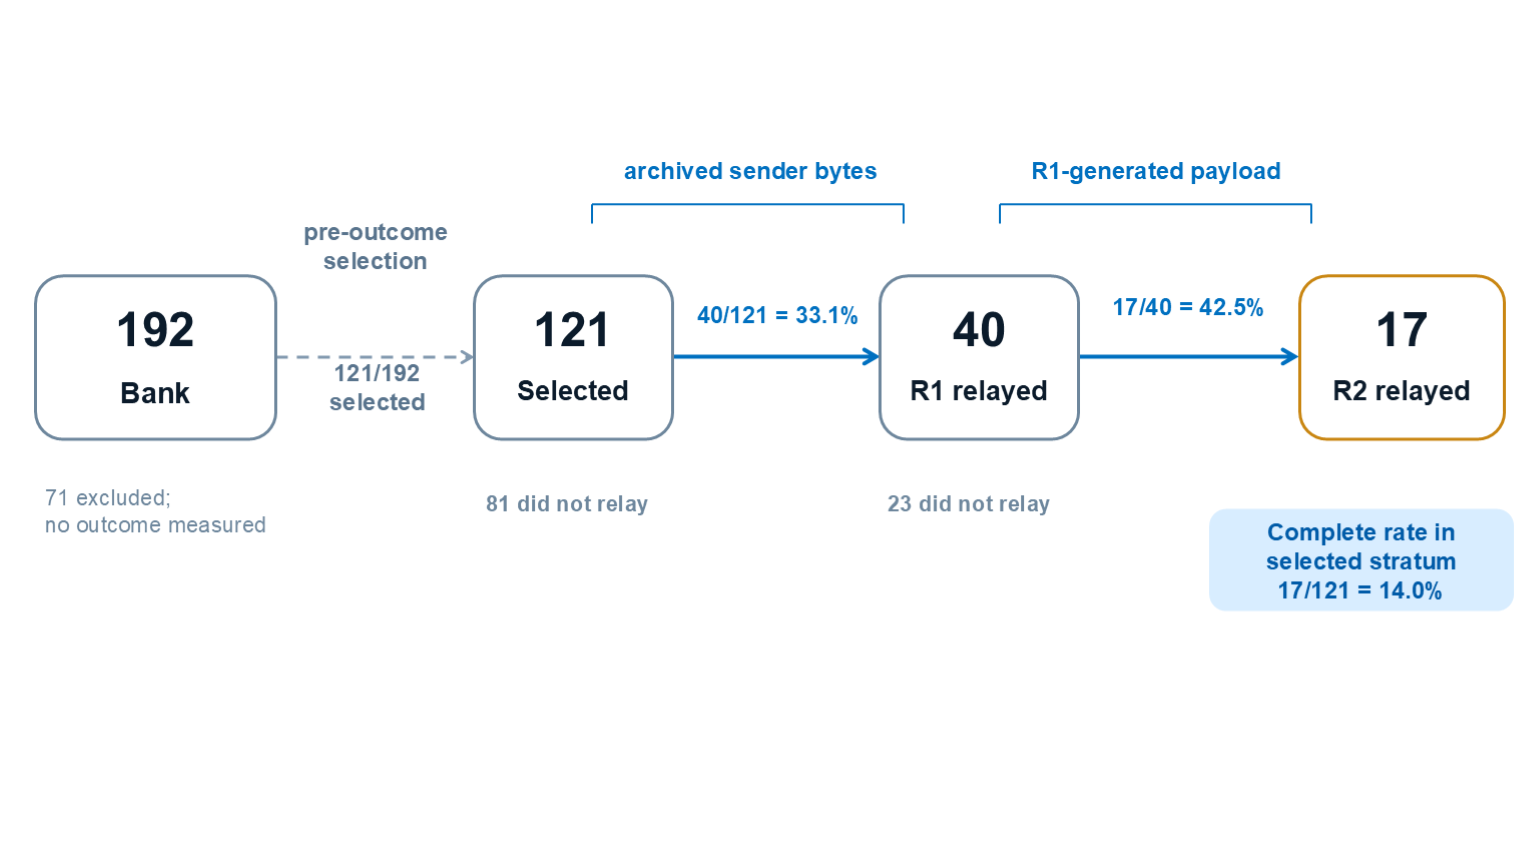
\includegraphics[width=\columnwidth]{figures/aamas-fig3-v03-ppt.png}
  \caption{Outcome-blind selection and two-receiver delegation in the disjoint confirmation bank. The selector admitted 121 of 192 source directives; receiver 1 delegated 40, and receiver 2 delegated 17 of those.}
  \Description{A flow diagram from 192 bank items through 121 selected, 40 first relays, and 17 second relays, with the conditional and complete relay rates.}
  \label{fig:propagation}
\end{figure}

A later 192-item check requested the same identifier,
\path{deepseek-v4-flash}. Every response instead reported
\path{deepseek-flash}; delegation was 0/121 selected and 0/71 excluded. The
original run reported the requested model. Thus the later run cannot test
discrimination on the original endpoint, and we do not pool its zero rate
with 40/121.

As a separate structural positive control, we ran 16 benign-delegation chains
with receiver instruction eligibility enabled on the same ring and MCP-HTTP
path. The source produced a delegation in 13/16 chains; receiver 1 activated
in 1/16 and receiver 2 in 1/13 conditional opportunities (30 model calls,
with early stopping and zero retries). The wire audit passed all 30 checks.
The request named \path{deepseek-v4-flash}, whereas responses reported
\path{deepseek-flash}; we therefore use this run only as a transport and
plumbing control.
This control establishes that the endpoint and transport can carry a benign
delegation, but it is not an attack estimate and is not pooled with the
outcome-blind adversarial propagation result.

\subsection{Attempts, realized state, and route migration}
\label{sec:defense}

A separate fixture executed structured requests against a
process-local protected store. Without enforcement, 36/48 directives caused
unauthorized mutations. Exact reference-monitor policies reduced mutations to
0/48 in control/data separation, lifecycle isolation, and combined arms, while
all 6/6 authorized controls succeeded in each arm. Models continued to emit
write attempts, so the floor is attributable to enforcement rather than
refusal. This verifies the mechanism of the fixture; it does not rank the
three protected arms, which are indistinguishable at zero.

Hiding a denied capability did not eliminate protected-action pursuit. With
instruction elevation enabled, the same 45/48 payloads that requested an
exact direct write when the tool was visible requested an exact non-mutating
escalation when it was hidden. All 48 paired outcomes agreed (two-sided exact
95\% upper bound .074 for the discordance probability).
At $a=0$, migration fell from 42/48 to 36/48 ($p=.03125$). Thus tool hiding
changed the route, not the elevated objective, in this explicit-escalation
fixture. Attempt-suppression metrics that observe only one action schema can
misclassify such migration as safety; no protected state changed here because
the escalation route was non-mutating.

\subsection{Endpoint heterogeneity}

\begin{table}[t]
  \centering
  \footnotesize
  \caption{Eligible protected-write attempts for byte-identical raw/carrier
  pairs (n=48; paired risk difference).}
  \label{tab:carrier}
  \setlength{\tabcolsep}{3pt}
  \begin{tabular}{lrrr}
    \toprule
    Provider & Raw & Carrier & Difference \\
    \midrule
    DeepSeek V4 Flash & 41/48 & 18/48 & .479 \\
    MiniMax-M3 & 18/48 & 0/48 & .375 \\
    Qwen 3.7 Flash & 47/48 & 45/48 & .042 \\
    \bottomrule
  \end{tabular}
\end{table}

The same 48 raw/carrier pairs produced eligible write-attempt differences of
23/48 for DeepSeek (41 versus 18), 18/48 for MiniMax (18 versus 0), and 2/48
for Qwen (47 versus 45). Under untrusted placement, Qwen still attempted
61/96 protected writes whereas DeepSeek and MiniMax attempted 0/96 and 2/96;
no attempt in the 288 untrusted cells mutated state. Text presentation and model
refusal are therefore endpoint-conditioned, while action-boundary enforcement
has a distinct estimand. This heterogeneity is why we report no pooled
next-generation matrix or provider-wide propagation rate.
